\documentclass{article}

\usepackage[english]{babel}
\usepackage[T1]{fontenc}
\usepackage[utf8]{inputenc}

\usepackage{longtable}
\usepackage{enumitem}
\usepackage{contour}
\usepackage{ulem}

\usepackage{amssymb}
\usepackage{algpseudocodex}

\usepackage{hyperref}
\hypersetup{colorlinks=true, linkcolor={black}, citecolor={black}}

\renewcommand{\ULdepth}{1.8pt}
\contourlength{0.8pt}

\newcommand{\myuline}[1]{%
  \uline{\phantom{#1}}%
  \llap{{#1}}%
}
\usepackage{gensymb}

\usepackage{lettrine}
\usepackage{ragged2e}
\usepackage{textcomp}

%\usepackage[dvipsnames]{xcolor}
\pagecolor{white}
\definecolor{sccomment}{RGB}{113, 113, 113}
\definecolor{scclass}{RGB}{38, 97, 177}
\definecolor{sclink}{RGB}{46, 21, 193}

\begin{document}

\begin{center}
\section*{\huge \sffamily Speculative Fractal Composition}

\texttt{\today}
\subsubsection*{Yann Ics\\Conceptual Composer\\\texttt{\small by.cmsc@gmail.com}}

\end{center}

\vspace{0.7cm}

\section*{Preamble}

Having missed the Call for Contributions to the Speculative Sound Synthesis Symposium 2024, I would like to bring my humble contribution. For the record, the \textit{Speculative Sound Synthesis} has started in November 2022 and will end in October 2025. The project is funded by the Austrian Science Fund (FWF) within the Programme for Arts-based Research (PEEK) – PEEK AR 713-G. It is hosted by the Institute of Electronic Music and Acoustics (IEM) at the University of Music and Performing Arts Graz.
\textit{The project’s aim is to generate aesthetic positions in the work with digital sound synthesis that open up speculative alternatives unreachable from standard positions}.\cite{iem}
Although it was more than likely my works do not fit this topic, as an oriented digital synthesis, or advancing coding, my point is a speculative thought about the music itself.

\smallskip

\noindent \rule{\linewidth}{.5pt}

\bfseries
\lettrine[lhang=.03]{T}{his} article aims, besides introducing and discussing some of my works, to overview my points concerning music as a concept, focusing on one aspect, fractality as a technical tool for composing, and how this can be speculative, as the art should be, beyond its potential or expected emotional response.

\mdseries

\bigskip
%++++++++++++++++++++++++++++++++++++++++++++++
%++++++++++++++++++++++++++++++++++++++++++++++

Being speculative in art relates to a hypothetical, futuristic, or imaginary outcome through (a) specific medium(s) -- involving most of the time interdisciplinarity such as science, sociology, and philosophy, to name the most common. This is expressed or covered in terms of concept.
The concept is a mind construction that allows one to name a state of knowledge that results in a set of epistemological relationships in a chain of signifieds and in a given context, particularly a cultural one.
Far from being frozen in time, the concept evolves and changes by using it, serving more to name an idea in its diversity than to describe an object in its uniqueness.

Music as a concept is a speculative object and does not exist as such in all cultures, and each culture, even each person has its own view of what is or what should be music.
The speculative perspective, besides describing or defining the object itself, aims to challenge conventional boundaries and more widely allows the exploration of possible futures through ineluctable or expected societal changes, with this intent in music to go further the experience itself, through or by composition, invention, and transmission of musical ideas.

The concept in music can be depicted thus as the frame in which music is possible often expressed in terms of structure or form. In this sense, the concept aims a result in or for a given situation.
Indeed, a piece of music can be the expression of several concepts as compositional or interpretive modalities. 

Like music, aesthetic is an elusive concept and by definition, speculative, but we can say that aesthetic tends towards a transcendent state or at least a certain satisfaction. Only, despite the strong subjectivity that aesthetic implies, both individually and collectively, this is highly related to the `zeitgeist'. It is a trend, shared more or less with our contemporaries, which was for instance a few decades ago more or less linked with noise music move and low-fi (still nowadays), indeed in their deepest understanding in terms of cognition\cite{mem}, algorithmic and synthesis. In this context, the aesthetic is not one of my purposes as such, but rather a way for questioning the listener about music as media understood as an extension of `Man'\cite{um}, through my quest of thinking and composing music otherwise.
\bigskip

%++++++++++++++++++++++++++++++++++++++++++++++
%  FRACTAL
%++++++++++++++++++++++++++++++++++++++++++++++

Music, like all things, is a process involving repetitions and variations. 
Of a usage without place or date, repetitions and variations are combined in various modalities, such as transpositions, symmetric transformations, and occasional or punctual rhythmic or pitch alteration, among others. 
Because the perception itself changes in time according to the context and the 'focus window' of the listener, strict repetition is only a view of the mind. Therefore, variations can take as many directions as contrasts or differences perceived as such.
Then, from micro variations to extreme contrasts, the field of possible paths is as large as the possible discretizations of the sonic phenomenon.

One of these approaches is to condition the entire structure by self-similarity by repeating a pattern, or profile, at various scales, dimensions, or levels.
It is from the sixteenth century we name the imitations of melody as a contrapuntal compositional technique the canon. In this paper, I focus on a particular case, known as the prolation canon, where imitations are carried out at different time scales\cite{fpm}. 
The systematization of this principle is called fractal. 
Although fractal is a relatively recent term defined by Mandelbrot in 1975\cite{bm} for a geometrical object that fulfills these criteria of self-similarity (strict replication at every scale), the term fractal as a system in music and in the time domain is in its sonification.
Nevertheless, in nature, although fractals are omnipresent, the self-similarity remains approximate because of the environmental constraints and, can be formalized otherwise like in biology such as a formal system called the Lindenmayer system based on grammar rules. 

Anyway, this work focuses on fractals as a self-similar pattern only, and it is the interpretation of each repeated pattern according to its position in time and dimension that determines its degree of variation if so. 

\bigskip

SuperCollider\cite{av}, as a programming language for real-time audio synthesis and algorithmic composition, is the perfect tool to manage fractals by coding the algorithm itself\cite[Section 6.3]{yx} as a class well-named \texttt{Fractal}\cite[\texttt{gsa.quark}]{yx} and managing its interpretation thanks to the flexibility of the coding. 

\bigskip

\begin{algorithmic}%[1]
\Procedure{fractal}{rtm, dur, rec, min, al | R, int}
\State
%\LComment{Require: \textnormal{min} $\in \mathbb{R}^{*+}$}
\If{R is nil} R $\gets$ rtm.normalizeSum*dur \EndIf
\If{int is nil} int $\gets$ \textsc{assoc}(rtm, al) \EndIf
\State tmp $\gets [\:]$ \Comment{for one dimension as sub-array of R}
\State 
\For{$i$ in R[0]} 
 \If{$ i=max$(R[0])} 
\State tmp $\gets$ rtm.normalizeSum*$i$
\Else $\;$ tmp $\gets$ $i$
\EndIf
\EndFor
\State
\If{rec $= 0$ \textbf{or} min $\geqslant min$(R[0])} 
\State \Return [R, int]
\Else  $\;$  
\If{rec $\in \mathbb{N}^+$} rec $=$ rec$-1$ \EndIf
\State \textsc{fractal}(rtm, dur, rec, min, al, 
        \newline \hspace*{5em} tmp.flat $\to$ R, 
        \newline \hspace*{5em} \textsc{assoc}(tmp, al) $\to$ int)
\EndIf
\EndProcedure
\State
\LComment{\textnormal{rtm} is a rhythm defined by a numerical array as a list of event's durations}
\LComment{\textnormal{dur} is the total duration}
\LComment{\textnormal{rec [optional]} is the number of dimensions or of recursions}
\LComment{\textnormal{min} is the minimal duration accepted which is required as \textnormal{min} $\in \mathbb{R}^{*+}$}
\LComment{\textnormal{al [optional]} is an associative list in the order of \textnormal{rtm}} %(if \textnormal{al} is nil then the new events according to the level of recursion are defined as $1$, if not as $0$)}
\end{algorithmic}

\bigskip

The algorithm itself is trivial, but this is the purpose of fractals. The complexity is closely related to the initial rhythm and the level of recursion, which (that level) is correlated with the duration of the piece and the value of the minimal duration. Complexity also depends on the interpretation in terms of synthesis parameters.

\begin{figure}[htbp]
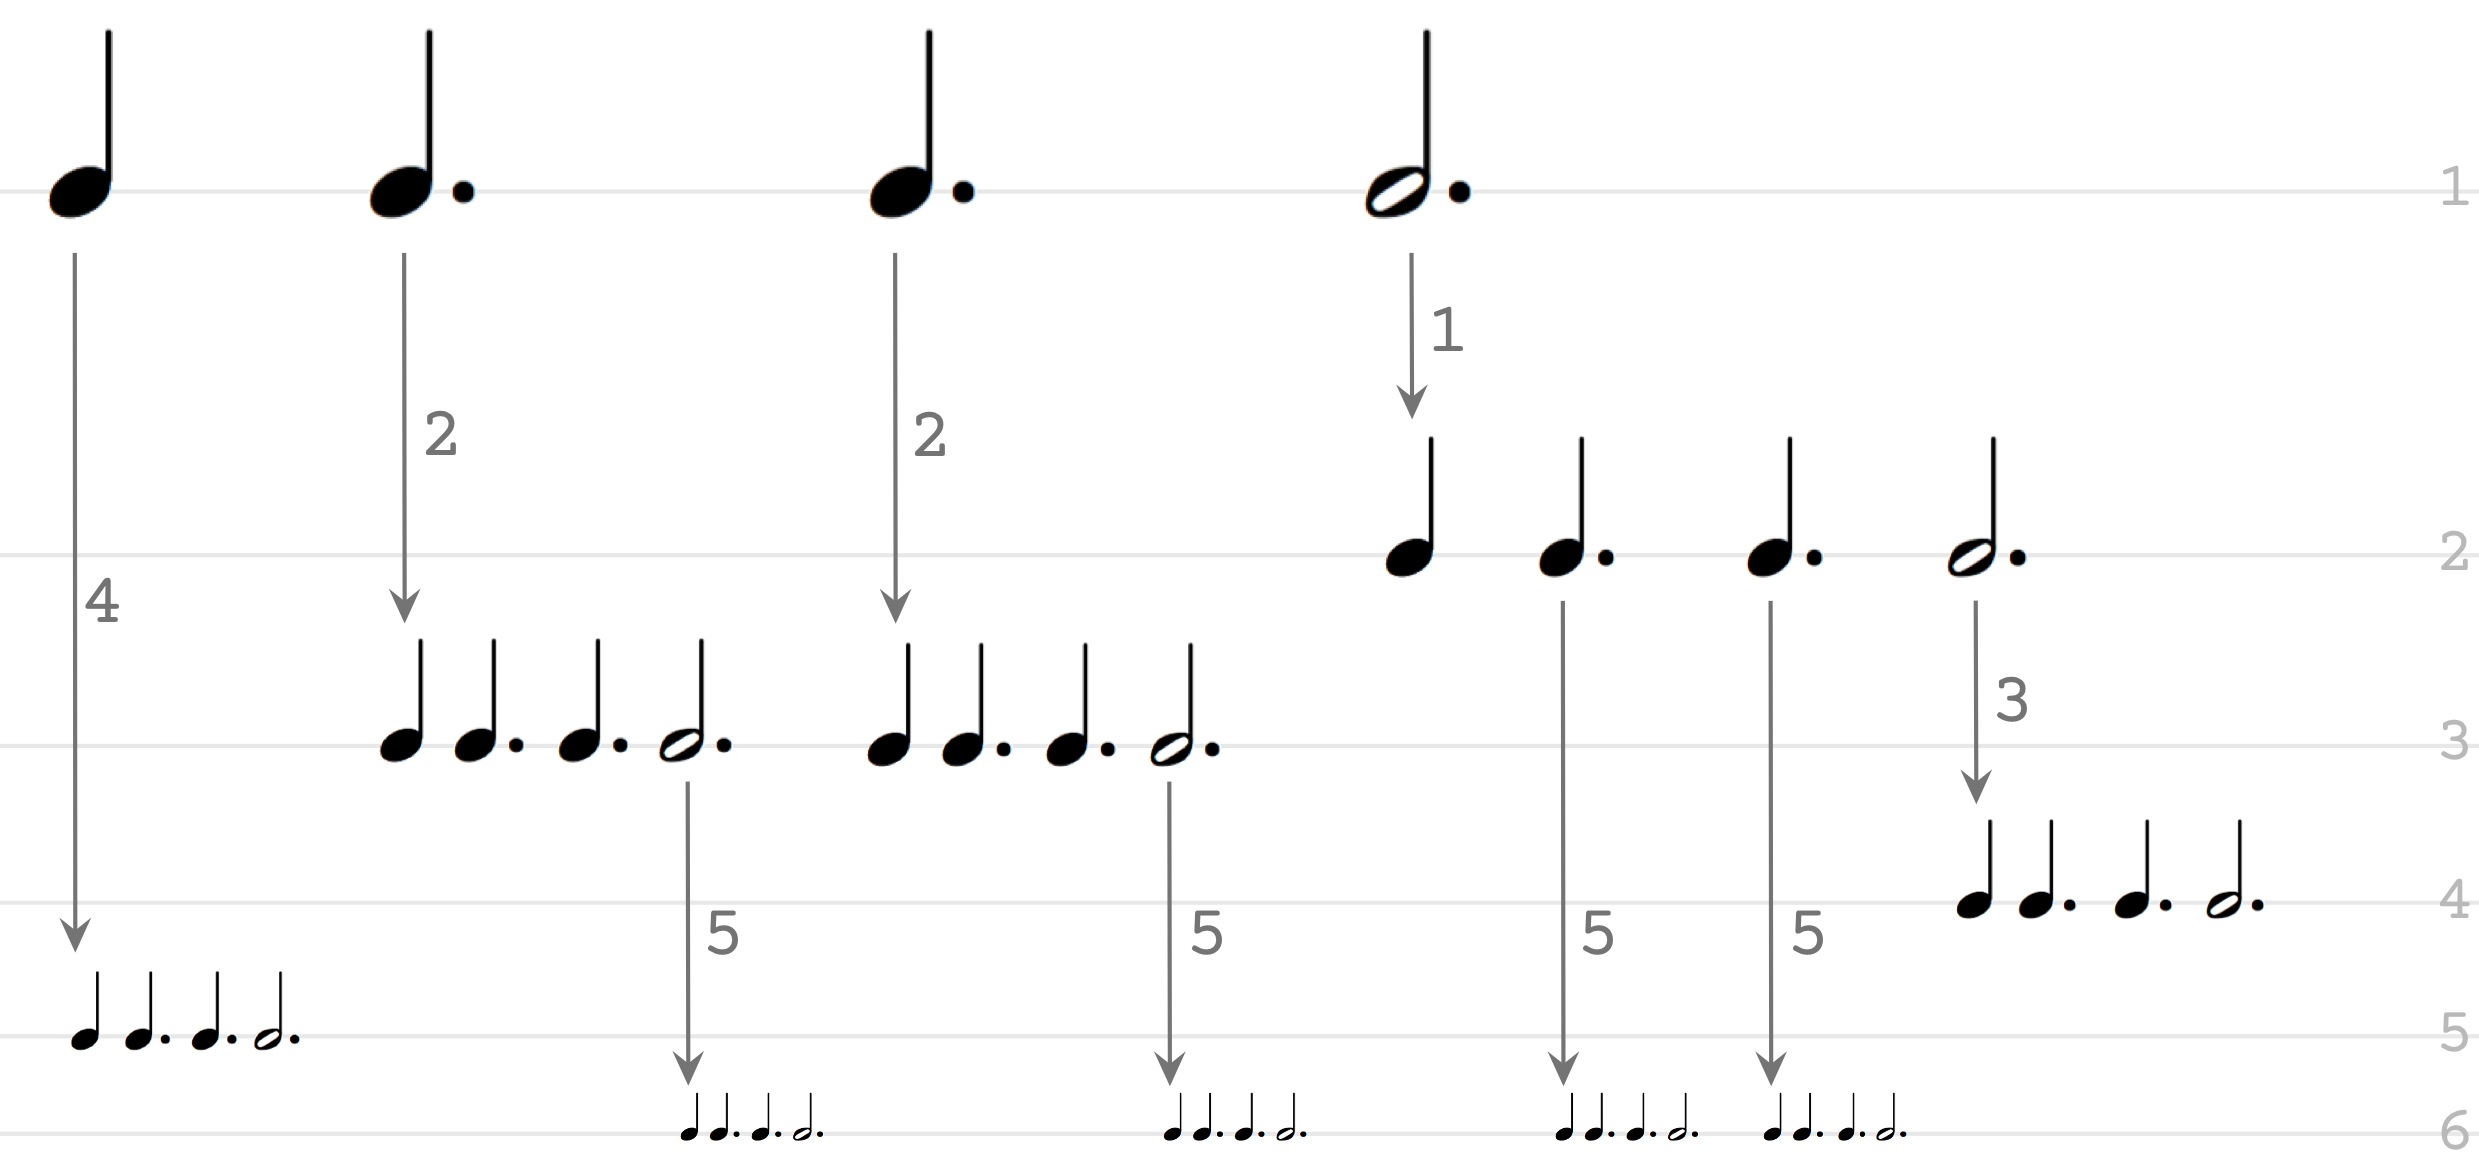
\includegraphics[width=\textwidth]{fractal}
\caption{\texttt{a = Fractal.newFrom([ 2, 3, 3, 6 ], rec:5)}}
\label{fractal}
\end{figure}

Note the function \textsc{assoc} which assigns for each duration in time their effectiveness as an array of 1 (or an event as an array) if so and as 0 (or a set of 0 according to the length of the event) if not. The events are grouped according to the initial dataset.

The figure \ref{fractal} illustrates the algorithm process using the code implemented in SuperCollider. In this instance, the number of dimensions defined by \texttt{a.depth} returns six as five recursions plus the `seed' (line 1). Figure \ref{score}   also shows the same fractal as a musical notation, like it can be heard as onset percussive triggers defined by \texttt{a.onsets}, according to the total duration of 14 seconds for this example (which is $2+3+3+6$ by default).

\begin{figure}[htbp]
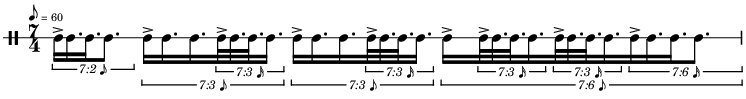
\includegraphics[width=\textwidth]{score}
\caption{Transcription of the figure \ref{fractal} considering only onsets.}
\label{score}
\end{figure}

The speculative fractal composition is a technical tool to structure music, a way to explore complex structures from simple ideas in order to manipulate sound at different levels related to its initial `axiom'. This can be seen precisely as a compromise between simplicity and complexity, an edge over which the funambulist composer evolves.
In my approach, different aspects of the fractal can be considered to structure the work as the level of recursivity, the synchrony superpositions, the ratios of the recursivity, with of course the related object of each event when it is provided, to name those I have implemented. Some randomness is also needed for specifically algorithmic music context to create more `musical' results, which can be related to the expressivity or something more `organic' in general terms. For written music, this can be equally a tool, a guideline, which must be adapted to fit the composer's musical intention.
 
\bigskip
Here is a list of my works using the SuperCollider class \texttt{Fractal}, illustrating some possible interpretations applied to it. 

\vspace{-2mm}

\subsection*{\texttt{HEX0} mvt 1 \textnormal{\cite[Section 8.2]{yx}}}
\vspace{-1mm}
According to a set of musical phrases, the fractality is applied to the well-known Risset Bell controlling its frequency and sustain, and the spatialization in terms of distance correlated with the level of fractality. The durations depend on a given ratio. 
\vspace{-1mm}

\subsection*{\texttt{DATA-01} part 3 \textnormal{\cite[Section 8.4]{yx}}} \vspace{-1mm}
From the contrastive analysis \cite[Section 4.4]{yx} applied to a given sound file, a deliberate substructure determines the fractal onsets, playing on the spatialization of streaming radio in terms of distance and panoramic, like the movie editing, from one shot to another according to a rhythm conducted by the said fractal onsets. 
\vspace{-1mm}

\subsection*{\texttt{105A1408} layer 2 \textnormal{\cite[Section 8.6]{yx}}}
\vspace{-1mm}
The fractal is applied to the identified recurrent patterns inside a given soundscape (according to the analysis \textsl{enkode} \cite[Chapter 1]{yx} involving only the duration and the centroid for each event) and chosen randomly for each initialization. A SuperCollider GUI \cite[Figure 8.11]{yx} controls also the presence in terms of distance for each dimension. 
Each onset triggers a percussive sample among a significative set. The centroids as data condition the rate of the samples. %Of course, the choice of the samples is decisive in this case. 

%++++++++++++++++++++++++++++++++++++++++++++++
%++++++++++++++++++++++++++++++++++++++++++++++
\bigskip

At the marge of and related to this work, I explored some ideas between the prolation canon and fractal that I called proportional canon. 
The main idea is to scale a given object according to an `attractor'  (which can be seen as a climax) and according to a given duration and ratio(s).
This object can be an array of durations or a sample as a sound file.
Also coded in SuperCollider context, the first one called \texttt{Canon}\cite[Section 6.2]{yx} is a class allowing two modalities, either by linear interpolation between the total duration and this duration multiplied by a given ratio or by the same ratio applied recursively on each voice. The position of the `attractor'  depends on this ratio which must be a number between 0 and 1 respectively excluded. The second one called \texttt{Sow}\cite[Section 7.4]{yx} is a \textsl{pseudo-UGen} applied to a sound file and played at different ratios. In this case, the position of the `attractor' is provided in second within the sample at ratio one.

Even though I experimented with the `proportional canon' in some of my works, there is no need to go further in detail because it is still very experimental and under development. Be that as it may, this remains relevant to mention here.

%++++++++++++++++++++++++++++++++++++++++++++++
%++++++++++++++++++++++++++++++++++++++++++++++

\section*{Discussion}

It is worth recalling the relevance of fractals in music, which remains a relatively frequent compositional modality, both intuitively and deliberately. Because as we know, repetition/variation is the very essence of music. Algorithms allow us to systematize this multidimensional approach and apply it to any compositional parameter. By coding, thanks to the SuperCollider concept, any pattern and recursivity can be managed independently to offer flexibility in terms of variations, opening a wide field of musical exploration, both experimental and research-based, including sound synthesis. 
%as the acquisition of knowledge based on heuristic perspectives
\bigskip

To finish my writing, I would like to mention an analytical tool I have elaborated on, which gives the possibility to retrieve fractalities of a given pattern inside a sequence using an algorithm called \texttt{differential-vector}\cite[Chapter 5]{yx}. This algorithm developed in Common Lisp compares two patterns defined by their respective durations and pitches (the latter can refer to any numerical coupled with the durations) and returns either a vector or the normalized norm of this vector. This estimates numerically the difference or the similarity between these two patterns according to the concordances on the onsets (time domain on the x-axis) and the profile (of the first derivative of the pitches or other profiles on the y-axis).
Then, if we apply this method to a whole sequence, by windowing according to a given length, we can detect the number and the position of each pattern matching the referent one, giving us an idea of redundancy of occurrence at different levels and different positions, as deliberate intent of the composer or as emergent phenomenon or surface structure, regardless all musical `decorations'. There exist biases, but this can be lessened with some settings of the algorithm, and according to the required relevance or accuracy of the analysis.

For instance, if we consider the fractal described in figure \ref{fractal}, based only on the differential durations, windowing from the length of the referent pattern to the size of the whole sequence, the algorithm returns six occurrences with a length of 4 at the indices 0, 7, 14, 19, 23, and 27, two occurrences with a length of 7 at the indices 4 and 11, one occurrence on 18 with 13, and one occurrence for the whole sequence.
Which match the accents of the transcription on the figure \ref{score}. The settings of the algorithm \texttt{differential-vector} are the output result as the vector of difference, the concordance on the x-axis according to the length of the referent (which means the minimal cardinal understood we check from this value, that is to say 4 in this instance), and a threshold of 0.001 because of rounded float numbers involved. The figure \ref{df} resumes the analysis.

\begin{figure}[htbp]
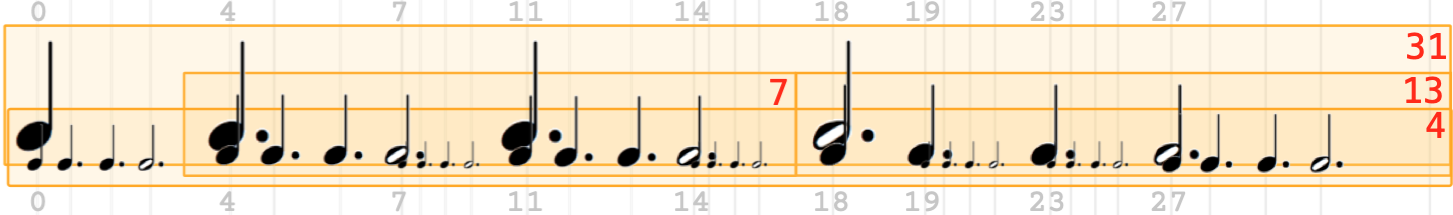
\includegraphics[width=\textwidth]{diff-vec}
\caption{Analysis in terms of redundancy with the Common Lisp algorithm \texttt{differential-vector} of the fractal sequence generated on figure \ref{fractal} in SuperCollider context.}
\label{df}
\end{figure}

This tool can be enhanced by extending the degrees of similarity or difference with a threshold applied to the durations, as long as these durations respect a proportional relationship in time. For instance, let $a$, $b$ and $c$ be the durations such as $a > b > c$ and $\epsilon$ the threshold (which should be expressed in percentage), then the rhythm $xyz$ which must be compared to the referent rhythm $bca$ must respect $z\pm\epsilon > x\pm\epsilon > y\pm\epsilon$ (work in progress).

\begin{thebibliography}{2}

\bibitem{iem}
	\textit{Speculative sound synthesis}. (n.d.). Speculative Sound Synthesis. Retrieved June 6, 2024, from
	\href{https://speculativesoundsynthesis.iem.sh}{\texttt{https://speculativesoundsynthesis.iem.sh}}

%\bibitem{yx}
%	Yann Ics. \textit{... à la recherche d'un nouveau paradigme de musique vivante}. Essay [draft], October 2023, online
%	\href{https://www.academia.edu/94964990}{\texttt{https://www.academia.edu/94964990}}

\bibitem{mem}
Bob Snyder, Robert Snyder,
\textit{Music and Memory: An Introduction},
A Bradford Book Mit Press, 2001.

\bibitem{um}
Marshall McLuhan,
\textit{Understanding Media -- The Extensions of Man},
First edition 1964, MIT Press edition, 1994.

\bibitem{fpm}
John McDonough, Andrzej Herczyński,
\textit{Fractal patterns in music},
Chaos, Solitons \& Fractals,
Volume 170,
2023. \\Online
\href{https://doi.org/10.1016/j.chaos.2023.113315}{\texttt{https://doi.org/10.1016/j.chaos.2023.113315}}

\bibitem{bm}
Benoit Mandelbrot,
\textit{Les objets fractals : forme, hasard et dimension}, (first edition 1975), Flammarion, 2010. 

\bibitem{av}
Andrea Valle,
\textit{Introduction to SuperCollider},
The MIT Press, 2016. \\Online
\href{https://www.academia.edu/114364804}{\texttt{https://www.academia.edu/114364804}}

\bibitem{yx}
	Yann Ics. \textit{Journal of Generative Sonic Art}. Articles/Reports, 2014--2024. Online
	\href{https://github.com/yannics/GSA/}{\texttt{https://github.com/yannics/GSA/}}
	\smallskip \\ \texttt{\textcolor{sccomment}{// install SuperCollider package gsa.quark}
	\\ \textcolor{scclass}{Quarks}.install(\textcolor{sclink}{"https://github.com/yannics/GSA/gsa"})}

%\bibitem{n3}
%	Yann Ics. \textit{Neuromuse3}. Artificial Intelligence Research -- Documentation, 2013--2024, online
%	\href{https://github.com/yannics/Neuromuse3/}{\texttt{https://github.com/yannics/Neuromuse3/}}
	
%\bibitem{yx}
%	Curtis Roads. \textit{Microsound}. MIT Press, 2004.\\ Online
%	\href{https://direct.mit.edu/books/book/3787/Microsound}{\texttt{https://direct.mit.edu/books/book/3787/Microsound}}

\end{thebibliography}

\end{document}